\documentclass[main.tex]{subfiles} % Subfile-Class


% ============================================================================== %
%                            Subfile document                                    %
% ============================================================================== %

\begin{document}

% Template

\subsubsection{Liniensensor}

Im folgenden Abschnitt ist die Entwicklung und Evaluierung eines Liniensensors
dokumentiert. Ziel ist es, einen einfach auszuwertenden Sensor zu entwickeln,
der das vorgegebene Klebeband (\textit{Tesa Gewebeband 4651}) problemlos vom Wettkampf-Untergrund unterscheiden kann.

% ===================================================================================
\paragraph{Anforderungen}

Das Klebeband muss auf einem rötlich
gefliessten Untergrund detektiert werden. Eine besondere Herausforderung
stellen hierbei längs und quer verlaufende Fliesenfugen dar, welche eine
ähnliche Farbe aufweisen. Dieser Untergrund ist in
Abbildung~\ref{fig:Untergrund_Wettkampf} gezeigt.

\begin{figure}[H]
    \centering
    \includegraphics[width=0.75\textwidth]{fig_Strecke_Tracken/Bild_Untergrund.jpg}
    \caption{Untergrund während des Wettkampfs}~\label{fig:Untergrund_Wettkampf}
\end{figure}

% ===================================================================================
\paragraph{Konzeptionierung}

\subsubsection{Aufbau und Auswertung}
Der Liniensensor wird aus acht einzelnen Messzellen aufgebaut. Es werden acht Messzellen
gewählt, damit eine möglichst breite Fläche durch den Sensor abgedeckt werden kann, aber
dennoch nicht zu viele Pins für die Auswertung benötigt werden. Dabei sollten stehts genau
zwei Messzellen direkt über dem Klebeband ausgerichtet sein. Jede einzelne Messzelle hat 
eine emittierende Diode und einen dazugehörigen Fototransistor. Je mehr Licht auf den 
Fototransistor einwirkt, desto höher ist der Strom, welcher durch ihn fliesst. Weil der 
Fototransistor als konstante Stromquelle interpretiert werden kann, wird der Spannungsabfall
über ihn ausgewertet. Ein hoher Strom durch den Phototransistor bewirkt einen hohen 
Spannungsverlust an einem davor geschaltenem Widerstand. Somit sollte die Spannung über dem
Fototransistor gegen Ground gezogen werden. Ist der Strom jedoch klein,
so fällt gemäss dem Ohmschen Gesetz wenig Spannung über dem Vorwiderstand ab was ein erhöhter
Spannungsabfall über dem Fototransistor zur folge hat. Diese Spannungen werden dann mittels einem
Analog-Digital-Wandler (ADC) ausgwertet.

% ======================================================================================
\subsubsection{Wahl des Lichtspektrums}
Damit der Unterschied zwischen dem Wettkampfuntergrund und dem Klebeband möglichst 
drastisch hervorgehoben werden kann, ist zuerst eine Evaluierung des optimalen
Lichtspektrums nötig. Im AnhangXXXXX sind Versuche dokumentiert, welche die Spannungen 
über dem Fototransistor im infrarotem Spektrum (IR) und im ultraviolettem Spektrum (UV) 
dokumentiert. Dabei wird für ersteres ein Emitter und ein Fototransistor im IR-Spektrum
verwendet. Beim Versuch im UV-Spektrum wird ein UV-Emitter mit einem Fototransistor 
im sichtbarem Spektrum verwendet. Dabei wird eine fluoreszierende Wirkung des Klebebandes 
vermutet. Gemäss der Dokumentation ist in der tat eine fluoreszierende Wirkung des Klebebandes 
ersichtlich und daraus folgt ein Spannungsunterschied über dem Fototransistor von Klebeband 
zu Wettkampfuntergrund um den Faktor 10. Aufgrund diesen deutlichen Ergebnissen wird auf ein 
UV-Emitter mit einem Fototransistor im sichtbaren Lichtspektrum zurückgegriffen.
In Abbildung~\ref{fig:Auswertung_Liniensensor} ist die Auswertung bildlich festgehalten.

\begin{figure}[H]
    \centering
    \includegraphics[width=0.5\textwidth]{fig_Strecke_Tracken/Auswertung_Liniensensor.pdf}
    \caption{Konzept der Auswertung mittels ADC}~\label{fig:Auswertung_Liniensesor}
\end{figure}

% ===================================================================================
\subsubsection{Geometrische Überlegungen}
Abbildung~\ref{fig:Konzept_graphml} zeigt die konzeptionelle Überlegungen einer Messzelle des
Liniensensor. Gemäss dem Datenblatt hat der UV-Emitter (Sender) einen Abstrahlwinkel von 15° und der
Fototransisor (Empfänger) einen Einfallswinkel von 60°. Diese Winkel und der festgelegte Abstand von 
Empfänger zu Sender definieren den Abstand der jeweiligen Messzellen untereinander sowie den
Abstand einer Messzelle zum Boden. Für eine möglichst störungsfreie Detektion muss auf dem Boden 
eine möglichst grosse Fläche des Empfänger-Kreises durch den Sender-Kreis ausgefüllt werden.\\
Diese einzelnen Messzellen sollen untereinander und von der Umwelt abgekapselt werden. Dies
mit der Begründung, dass die Fototransistoren, gegebenenfalls empfindlich auf
Umwelteinflüsse reagieren könnten. Daher wird ein Gehäuse für die Abschirmung von Umwelteinflüssen
notwendig.

\begin{figure}[H]
    \centering
    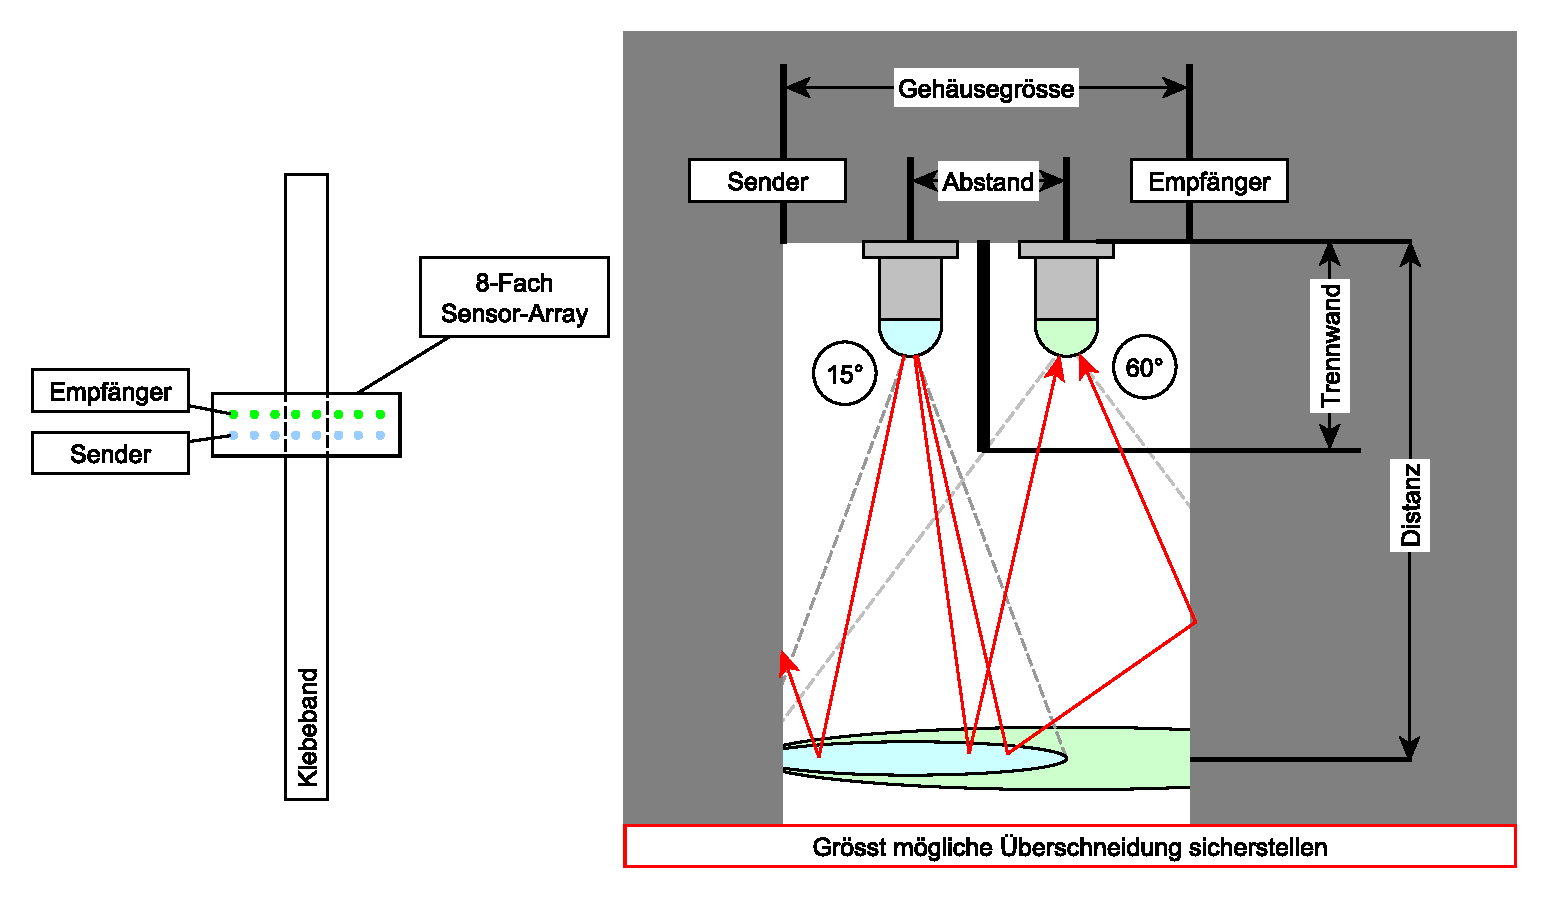
\includegraphics[width=0.75\textwidth]{fig_Strecke_Tracken/Konzept.pdf}
    \caption{Konzept des Liniensensors}~\label{fig:Konzept_graphml}
\end{figure}
% ===================================================================================
\subsubsection{Positionierung der Komponenten}
!!!!!!Überarbeiten, weil ausstrahlwinkel anderst!!!!!!!!
In diesem Abschnitt wird die optimale Positionierung der Sender und Empfänger ermittelt.\\ 
Der Abstand zwischen einem Sender und einem Empfänger wird aufgrund der Bauform beider 
Komponenten bestimmt.
Beide Komponenten besitzen das gleiche Gehäuse. Gemäss Datenblatt ist der Durchmesser
beider Komponenten mit Herstellertoleranz maximal 4mm. Es folgt eine Berechnung des 
Mindestabstand beider Komponenten. Das Mass bezieht sich auf die Mitte der beiden 
Komponenten, wie in Abbildung~\ref{fig:Konzept_graphml} dargestellt.
\[ X_{min} = \frac{D_s}{2} + \frac{D_e}{2} = \frac{4mm}{2} + \frac{4mm}{2} = 4\,\text{mm} \]
Damit genügend Reserve vorhanden ist, wird ein Abstand von 4.6mm zwischen Sender und
Empfänger in einer Messzelle gewählt.\\

Folglich wird der Abstand zwischen einer Messzelle und dem Boden ermittelt. Dafür 
wird die Beziehung der beiden Radien ausgenutzt, welche bei der zu ermittelnden Höhe
h auf den Boden gestrahlt werden. Es folgt also:

\[
R_s = \tan(\alpha) \cdot h 
\]
\[
R_e = \tan(\beta) \cdot h
\]

Nun kann \( R_e \) auch durch \( R_s \) und den Mindestabstand \( X_{min} \) formuliert werden:
\[
    R_e = R_s + X_{min}
\]
Nun wird \( R_s \) und \( R_e \) eingesetzt und nach h aufgelöst:
\[
h = \frac{4.6}{\tan(\beta) - \tan(\alpha)} = \frac{4.6mm}{\tan(30^\circ) - \tan(7.5^\circ)} = 10.32{mm} \approx 10{mm}
\]

Aufgrund 15 anstatt 30 Abstrahlwinkel stimmt der abstand zweier Messzellen nicht mehr.
!!!!!Messzellenabstand irgenwie begründen!!!!!


% ===================================================================================

\subsubsection{Dimensionierung Gehäuse}
!!!!!!!!Daten aus Test benötigt!!!!!!!\\
Damit der Empfänger möglichst wenig auf Umwelteinflüsse reagiert, wird nun ein 
Gehäuse dimensioniert, welches den Sensor abschirmen soll. Die nachfolgende 
Abbildung~\ref{fig:Gehaeuse_Vermasst} zeigt eine Skizze, welche den Aufbau des Gehäuses repräsentiert.
Die isometrische Ansicht des Gehäuse ist in Abbildung~\ref{fig:Gehaeuse_Isometrisch}



\begin{figure}[H]
    \centering
    \includegraphics[width=0.75\textwidth]{fig_Strecke_Tracken/Gehaeuse_Vermasst.pdf}
    \caption{Vermassung des Gehäuses in Siemens NX}~\label{fig:Gehaeuse_Vermasst}
\end{figure}

\begin{figure}[H]
    \centering
    \includegraphics[width=0.75\textwidth]{fig_Strecke_Tracken/Gehaeuse_Isometrisch.pdf}
    \caption{Isometrische Ansicht des Gehäuses in Siemens NX}~\label{fig:Gehaeuse_Isometrisch}
\end{figure}



% ===================================================================================

\subsubsection{Elektrotechnische Dimensionierung}

\begin{figure}[H]
    \centering
    \includegraphics[width=0.5\textwidth]{fig_Strecke_Tracken/Schema_Messzelle_Liniensensor.pdf}
    \caption{Schema einer Messzelle}~\label{fig:Messzelle}
\end{figure}

Abbildung~\ref{fig:Messzelle} zeigt das Schema einer einzelnen Messzelle. Die Speisung von 5V für 
den UV-Emitter ist notwendig, weil gemäss Datenblatt eine Spannung von 2.9V bis 3.5V abfällt. Daher reicht
eine Speisung von 3.3V nicht aus. Ausserdem wurde als Sicherheitsmassnahme beim Messabgang über dem 
Fototransistor ein Platz für ein Widerstand eingebaut, damit bei allfälligen Stromspitzen der Strom 
limitiert werden könnte. Weil dies aber mit der verwendeter Auswertung nicht notwendig ist, wird ein
null ohm Widerstand eingebaut. Die Potentiometer werden eingebaut, dass allfällige Bauteiltoleranzen
eliminiert werden können. Im Anhang!!!!!!!! wird dargestellt, wie die Werte der Komponenten R1.1, Rp1 und R1.3 
Dimensioniert werden.\\\\




% ===================================================================================


\subsubsection{Liniensensor als PCB}

Damit der Liniensensor möglichst praxisnahe getestet 
werden kann, wurde dieser als PCB mit dem CAD-Tool Kicad erstellt. Dabei wurden die 
oben formulierten Anforderungen und Dimensionierungen eingehalten. In Abbildung~\ref{fig:Liniensensor_Top} 
ist die Draufsicht und in Abbildung~\ref{fig:Liniensensor_Bottom} die Untersicht dargestellt.

\begin{figure}[H]
    \centering
    \includegraphics[width=0.75\textwidth]{fig_Strecke_Tracken/Liniensensor_Top.pdf}
    \caption{Liniensensor in Kicad von oben}~\label{fig:Liniensensor_Top}
\end{figure}

\begin{figure}[H]
    \centering
    \includegraphics[width=0.75\textwidth]{fig_Strecke_Tracken/Liniensensor_Bottom.pdf}
    \caption{Liniensensor in Kicad von unten}~\label{fig:Liniensensor_Bottom}
\end{figure}




% ===================================================================================

\paragraph{Versuche}
Es wurde überprüft, welches Lichtspektrum am besten geeignet sind und die verschiedenen Ströme
durch den Fototransistor wurden getestet. Ausserdem wurde im UV-Spektrum die Spannungen über dem Fototransistor
gemessen. Mittels einem 
Arduino wurden für einen Test alle Eingänge ausgewertet und der Liniensensor validiert. 
Alle Messungen sind im Anhang dokumentiert.

% ===================================================================================
\paragraph{Entscheidung und Fazit}
Aufgrund der grossen Spannungsdifferenz zwischen Klebeband und Fliese/ Fuge, wurde eine mögliche
fluoreszierende Wirkung des Klebebandes im UV-Spektrum bestätigt. Durch die Messungen wurde das 
Konzept des Liniensensors überprüft und validiert. Dieses Prinzip kann im Projekt angewendet
werden.

\end{document}
